\section{案例研究:Salsa 和 ChaCha PRG}\label{sec:3-6}

在实践中,有许多建立PRG和流密码的方法。一种方法是使用 \ref{subsec:3-4-2} 小节中介绍的Blum-Micali 范式来构建 PRG。另一种方法,我们将在第\ref{chap:5}章中介绍,它用一种更加通用的,称作伪随机函数的原语在计数器模式下构建 PRG 和流密码。我们下面介绍一种使用后者的实际构造。

Salsa20/12 和 Salsa20/20 是由丹尼尔·伯恩斯坦于 2005 年设计的快速流密码。Salsa20/12 是被选入 eStream 流密码组合的四种Profile 1 流密码之一。eStream 是一个选定适合实际使用场景的快速安全的流密码的项目。伯恩斯坦又于 2008 年提出了Salsa20/12 和 Salsa20/20 的变体,分别被称作 ChaCha12 和 ChaCha20。这些流密码已被纳入一些广泛部署的协议,如 TLS 和 SSH。

\begin{figure}
  \centering
  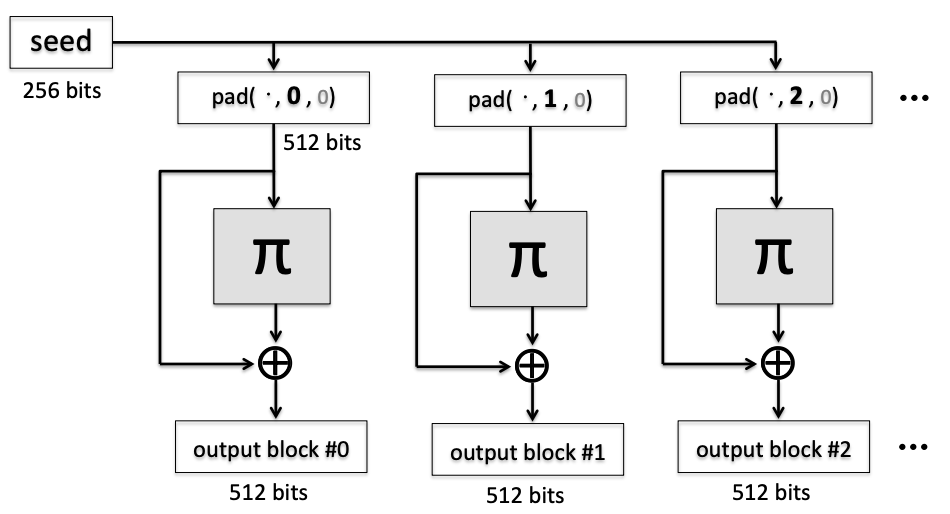
\includegraphics[width=0.7\linewidth]{figures/chapter3/fig8.png}
  \caption{Salsa 和 ChaCha PRG 的示意图}
  \label{fig:3-8}
\end{figure}

让我们先简单介绍一下 Salsa 和 ChaCha 流密码家族的底层 PRG。这些 PRG 将一个 $256$ 比特种子和一个 $64$ 比特的 nonce 作为输入。现在我们忽略 nonce,先简单地将其设置为 $0$,我们会在本节末尾讨论 nonce 的作用。Salsa 和ChaCha PRG 都遵循图 \ref{fig:3-8} 所示的顶层设计结构。它们都包含两个组件:
\begin{itemize}
	\item 一个填充函数 $\mathrm{pad}(s,j,0)$,将$256$比特的种子$s$和$64$比特的计数器$j$结合,形成一个$512$比特的分组。第三个输入是一个$64$比特的 nonce,我们目前先把它置为$0$。
	\item 一个固定、公开的置换 $\pi:\{0,1\}^{512}\to\{0,1\}^{512}$。
\end{itemize}
这两个组件使用以下算法(见图 \ref{fig:3-8})输出 $L<2^{64}$ 个伪随机分组,每个分组$512$比特长:

\vspace*{5pt}

\hspace*{5pt} 输入:种子$s\in\{0,1\}^{256}$\\
\hspace*{26pt} 1. 对于 $j\leftarrow0$ 到 $L-1$:\\
\hspace*{26pt} 2. \quad\quad\quad$h_j\leftarrow\mathrm{pad}(s,j,0)\in\{0,1\}^{512}$\\
\hspace*{26pt} 3. \quad\quad\quad$r_j\leftarrow\pi(h_j)\oplus h_j$\\
\hspace*{26pt} 4. 输出 $(r_0,\dots,r_{L-1})$。

\vspace*{5pt}

\noindent
最终的 PRG 输出是 $512\cdot L$比特长的序列。我们注意到,在 Salsa 和 ChaCha 中,第 3 行中的异或运算是一个稍微复杂的操作:512比特的操作数$h_j$和$\pi(h_j)$被分成$16$个字,每个字长$32$比特,然后逐字计算模$2^{32}$加法。

Salsa 和 ChaCha 的设计是高度可并行的,并且可以利用多处理器核心来加快加密速度。此外,它还能实现对输出分组的随机访问:想要输出分组的编号$j$,并不需要先把所有前序分组都计算出来。基于 Blum-Micali 范式的生成器则不具备这些特性。

我们将在下一章的练习 4.23 中分析 Salsa 和 ChaCha 的安全性,为此我们还需要一些其他的工具。

\begin{snote}[一些细节。]
我们下面简单介绍填充函数 $\mathrm{pad}(s,j,n)$ 和 ChaCha20 中使用的置换 $\pi$。填充函数的输入是一个$256$比特的种子$s_0,\dots,s_7\in\{0,1\}^{32}$,一个$64$比特的计数器$j_0,j_1\in\{0,1\}^{32}$和一个$64$比特的 nonce $n_0,n_1\in\{0,1\}^{32}$。它输出一个$512$比特的分组,表示为$x_0,\dots,x_{15}\in\{0,1\}^{32}$。输出被组织为一个由$32$比特长的字所构成的$4\times4$矩阵,如下所示:
\begin{equation}
\begin{pmatrix}
x_0 & x_1 & x_2 & x_3 \\
x_4 & x_5 & x_6 & x_7 \\
x_8 & x_9 & x_{10} & x_{11} \\
x_{12} & x_{13} & x_{14} & x_{15}
\end{pmatrix}
\longleftarrow
\begin{pmatrix}
c_0 & c_1 & c_2 & c_3 \\
s_0 & s_1 & s_2 & s_3 \\
s_4 & s_5 & s_6 & s_7 \\
j_0 & j_1 & n_0 & n_1
\end{pmatrix}
\end{equation}
其中$c_0,c_1,c_2,c_3$是固定的$32$比特常数。

置换 $\pi:\{0,1\}^{512}\to\{0,1\}^{512}$ 是通过对一个简单的置换进行固定次数的迭代来实现的。$\pi$的$512$比特输入被当作一个由$32$比特的字构成的$4\times4$数组,记作$x_0,\dots,x_{15}$。在 ChaCha20 中,函数$\pi$是通过重复10次以下步骤来实现的:
\begin{center}
\begin{tabular}{ll}
 (1) $\mathrm{QuarterRound}(x_0,x_4,x_8,x_{12})$, & (2) $\mathrm{QuarterRound}(x_1,x_5,x_9,x_{13})$,\\ 
 (3) $\mathrm{QuarterRound}(x_2,x_6,x_{10},x_{14})$, & (4) $\mathrm{QuarterRound}(x_3,x_7,x_{11},x_{15})$,\\  
 (5) $\mathrm{QuarterRound}(x_0,x_5,x_{10},x_{15})$, & (6) $\mathrm{QuarterRound}(x_1,x_6,x_{11},x_{12})$,\\
 (7) $\mathrm{QuarterRound}(x_2,x_7,x_8,x_{13})$, & (8) $\mathrm{QuarterRound}(x_3,x_4,x_9,x_{14})$\\
\end{tabular}
\end{center}
这里,$\mathrm{QuarterRound}(\texttt{a},\texttt{b},\texttt{c},\texttt{d})$的定义可参见下面的C程序所表示的步骤:
\begin{center}
\begin{tabular}{lll}
\texttt{a += b;} & \texttt{d \^{}=  a;} & \texttt{d <<<= 16;}\\
\texttt{c += d;} & \texttt{b \^{}=  c;} & \texttt{b <<<= 12;}\\
\texttt{a += b;} & \texttt{d \^{}=  a;} & \texttt{d <<<= 8;}\\
\texttt{c += d;} & \texttt{b \^{}=  c;} & \texttt{b <<<= 7;}
\end{tabular}
\end{center}
注意到QuarterRound的前四个调用,即步骤(1-4),从左到右分别应用于$4\times4$矩阵的四列上。接下来的四次调用,即步骤(5-8),分别应用于矩阵的四条对角线。这就完成了我们对 ChaCha20 的描述,只是我们还需要讨论一下 nonce 的使用。
\end{snote}

\begin{snote}[使用nonce。]
虽然我们到目前为止讨论的 PRG 只把种子作为输入,但在实践中使用的许多 PRG 还需要一个额外的输入,称为\emph{nonce}。也就是说,PRG 是一个函数 $G:\mathcal{S}\times\mathcal{N}\to\mathcal{R}$,其中$\mathcal{S}$和$\mathcal{R}$和之前一样,而$\mathcal{N}$被称为\emph{nonce 空间}。nonce 能让我们由一个种子 $s$ 产生多个伪随机输出。也就是说,$G(s,n_0)$ 是一个伪随机输出,而当$n_1\neq n_0$时,$G(s,n_1)$ 就是另一个伪随机输出。nonce 将 PRG 变成了一个更强大的原语,称为\emph{伪随机函数(pseudo-random function)},我们将在下一章更详细地讨论它。正如我们将看到的,安全的伪随机函数能让我们使用同一个种子安全地加密多条消息。
\end{snote}